%************************************************
\chapter{Implementation}\label{ch:implementation}
%************************************************
In order to validate the metric, an application that appealed both to developers as well as employers needed to be built. It should motivate developers enough to grant it access to their public repositories, and convince recruiters to use it. The special means that the development of the application required will be described in this chapter.

\section{Architecture}
Web applications are state-of-the art as they require little servicing and no complex versioning. Our use case of many users taking advantage of a common dataset is perfect for this architecture. We decided to implement the serverside logic in Node.js, which is a JavaScript runtime. The client-side runs in the browser and makes use of standard web technologies like CSS3, HTML5 and Javascript. The analysis results are saved in a SQLITE3 database.
\newline

The serverside part needs to master two tasks: serving data to clients as well as analyzing repositories from developers. These are two very different concerns. In order not to stall one of the tasks while executing the other, we decided to have two dedicated processes running alongside each other. One of these will serve the data and perform queries on the database, while the other will keep the local copies of repositories up to date and build the metric on them. We will call the first component the \textit{hirebot} and the latter the \textit{analyzer}.

\subsection{Database schema}
The database schema of hirebot is not very complex. Users are central to the application and every other type of data is associated with one, as seen in figure \ref{fig:schema}. Basic data retrieved from the GitHub API is saved as well as the values generated from the repositories.

\subsection{Hirebot}
The component that plays the webserver role is called \textit{hirebot}. It handles the usual webserver tasks like formatting templates and querying the database for answering HTTP requests to an endpoint.
\newline

Additionally it implements the foundation for data analysis. It allows developers to register with GitHub to grant the application access to their emails and their repositories. Hirebot then notifies the analyzer, which goes on to clone and analyze the repositories. This process is also depicted in figure \ref{fig:regprocess}.

\begin{figure}[ht]
  \centering
  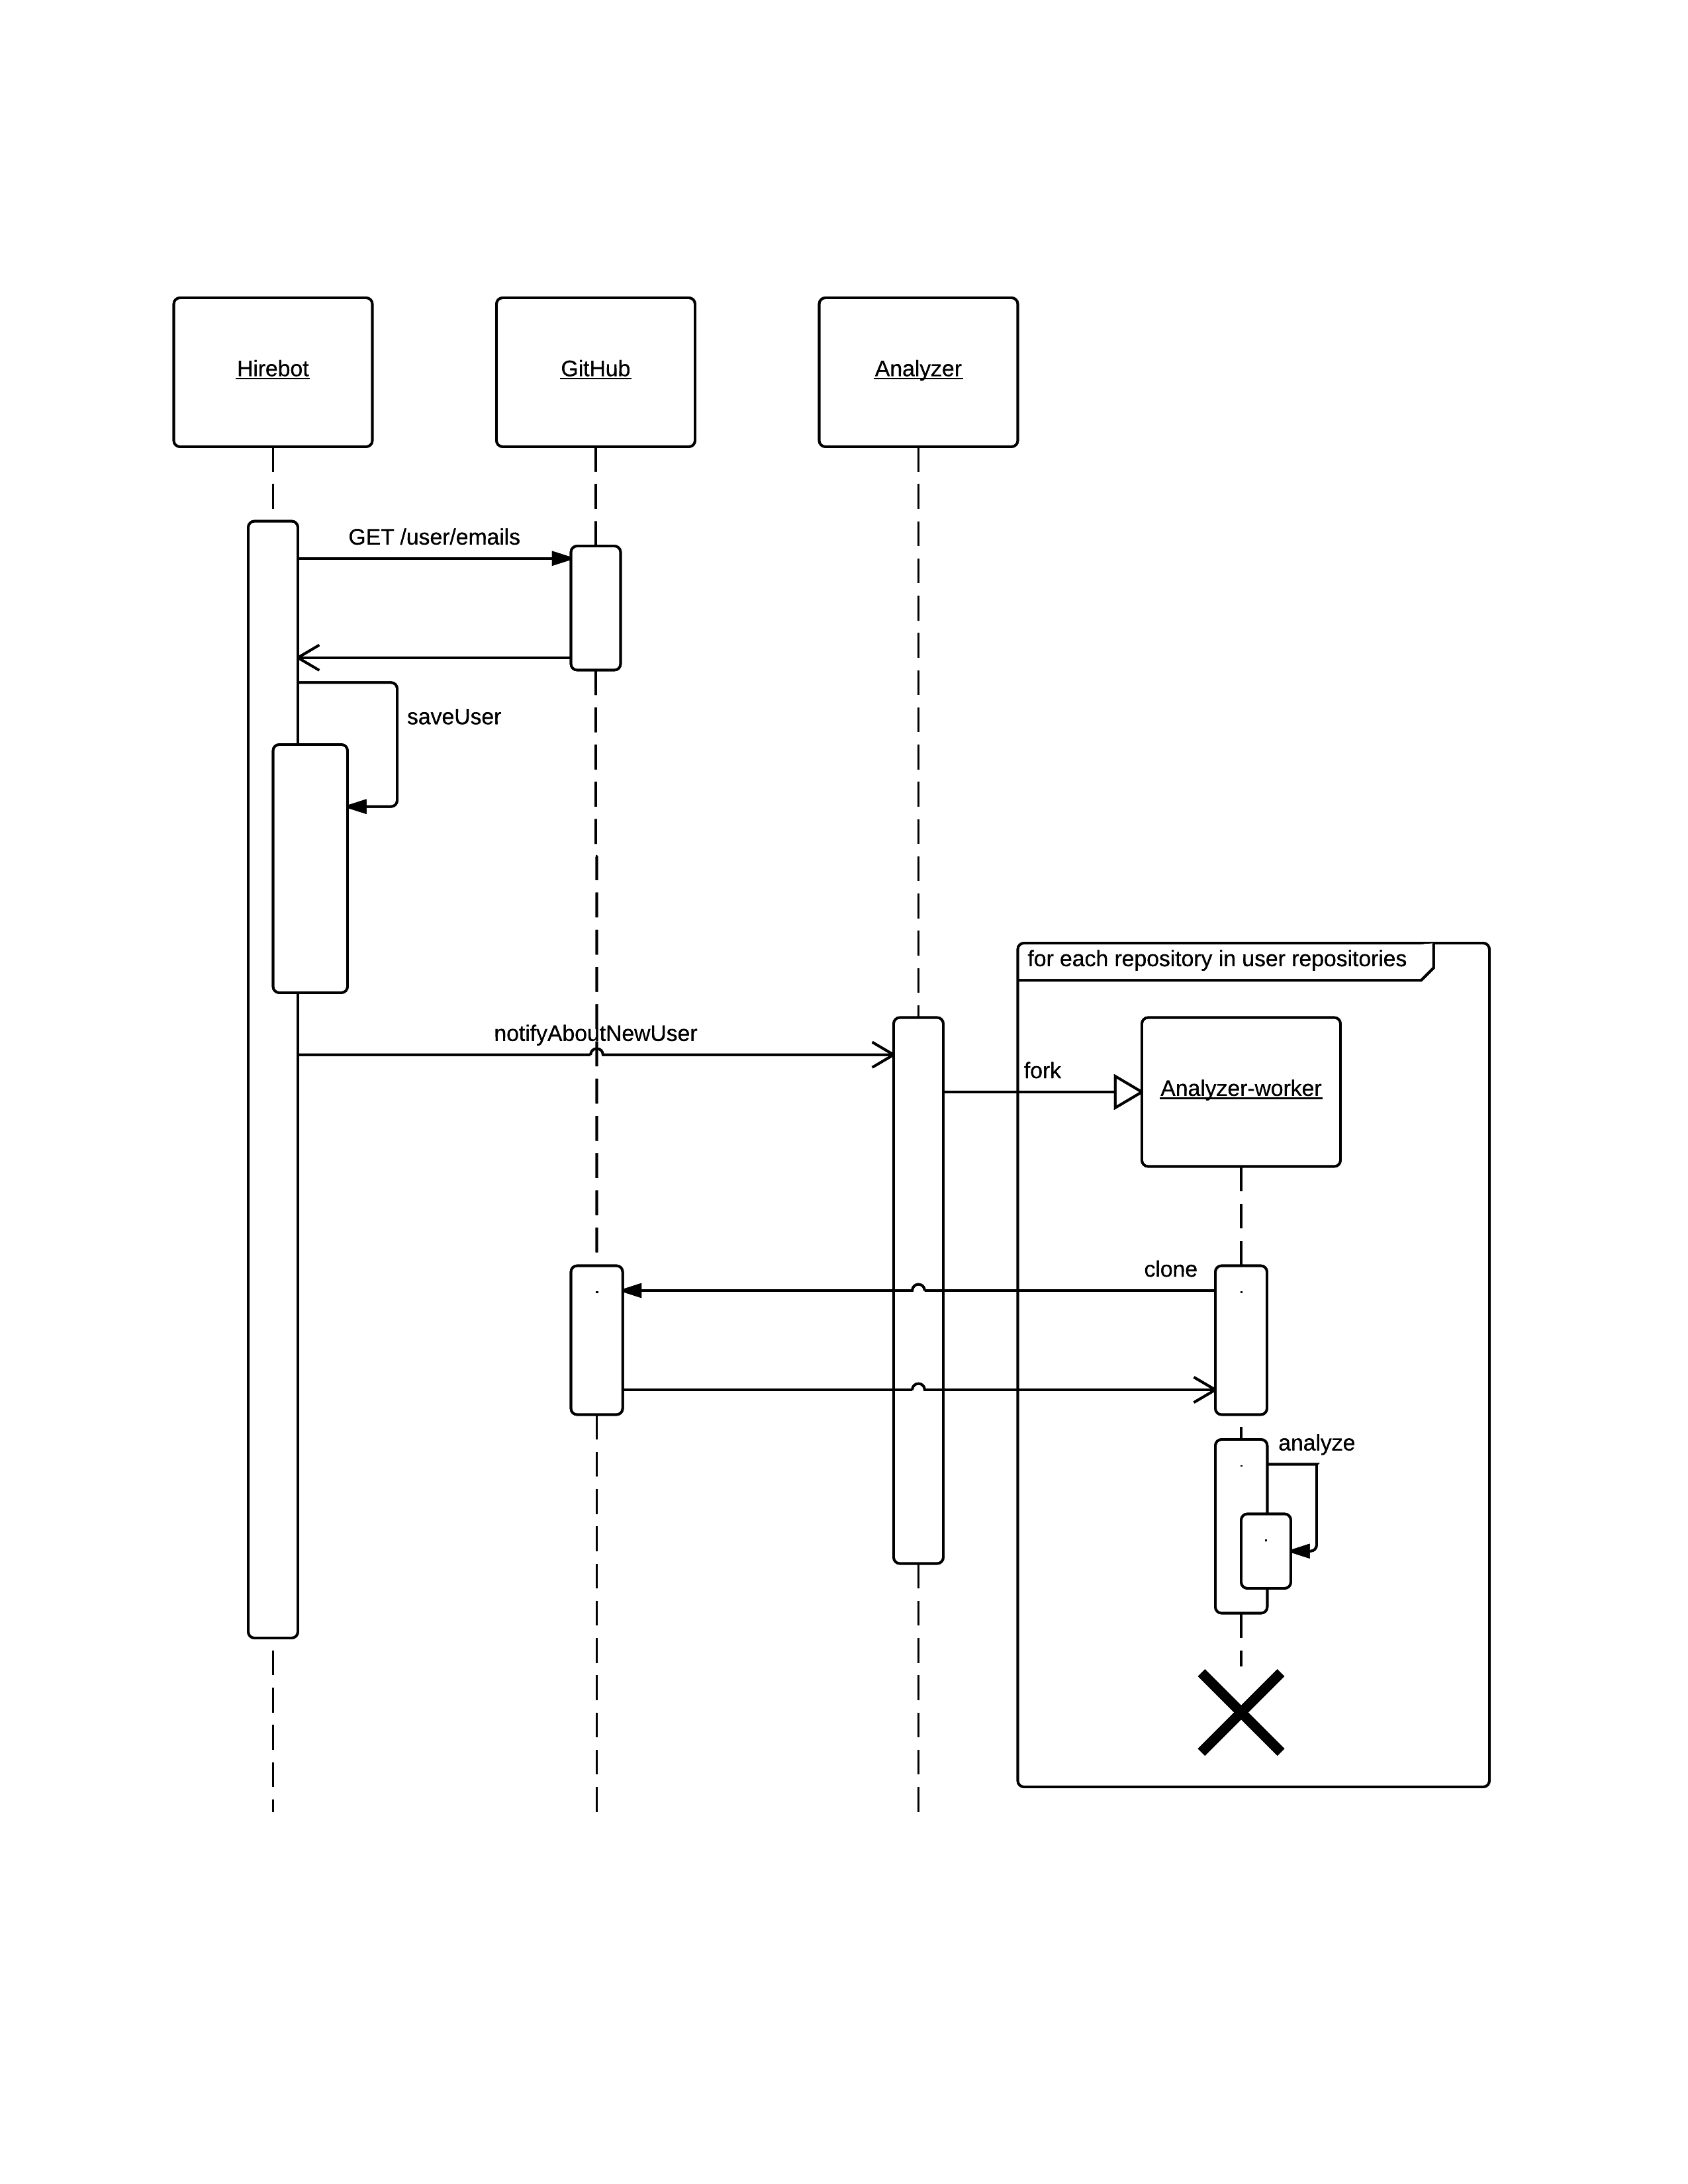
\includegraphics[width=35em]{gfx/registersequence.png}
  \caption{The interplay of the three processes with the GitHub API after the OAuth 2.0 dance has been completed.}
  \label{fig:regprocess}
\end{figure}

\subsection{Analyzer}
The analyzer component of the application handles two slightly different
tasks. First, it has to schedule an initial clone of all repositories
a user owns upon his registration. Then, it has has to keep those local
copies up to date and add new repositories, both in a recurring fashion.


These are certainly no impossible tasks, but \textit{nodegit}, the library
that was used for accessing the git repository data, was
leaking memory strongly and to counter this, a sub-process structure was
implemented. The analyzer itself only executes management logic,
schedules the analysis, and communicates with the hirebot process.
For executing the analysis, it forks an \textit{analyzer-worker} for each
single repository. The worker clones or updates that repository,
runs the analysis, saves the results into the database and terminates
upon completion. The forks are done sequentially to avoid putting
too much load on the system at once, but could be done in parallel as well.

\subsection{Metric implementation}\label{sec:metric-implementation}
The metric described in section \ref{sec:technicalfit} is fully implemented in the analyzer-worker component. Its implementation works on a per-repository basis and can be written down like this:

\begin{lstlisting}[frame=false]
for c:=mostRecentlyAnalyzedCommit to lastCommit do
  for d:= c.firstDiff to c.lastDiff do
    var language = determineFileLanguage(d.file)
    var lineCount = d.lineCount
    saveExperience(language, c.id, c.date, lineCount)
\end{lstlisting}

Additionally, a special JavaScript analyzer was built into the algorithm.
It adds McCabe and Halstead complexity metric information about single
commits. Thus, the final implementation amounts to:

\begin{minipage}{\linewidth}
\begin{lstlisting}[frame=false]
for c:=mostRecentlyAnalyzedCommit to lastCommit do
  for d:= c.firstDiff to c.lastDiff do
    var language = determineFileLanguage(d.file)
    var lineCount = d.lineCount
    saveExperience(language, lineCount)

    if language == 'JavaScript'
      var fileContentsBeforeCommit = d.file.contents
      var fileContentsAfterCommit  = d.parent.file.content

      var mcCabeComplexityBefore = getMcCabeComplexity(fileContentsBeforeCommit)
      var mcCabeComplexityAfter = getMcCabeComplexity(fileContentsAfterCommit)
      var halsteadComplexityBefore = getHalsteadComplexity(fileContentsBeforeCommit)
      var halsteadComplexityAfter = getHalsteadComplexity(fileContentsAfterCommit)

      saveJavaScriptMeasures(c.id, c.date, mcCabeComplexityBefore,mcCabeComplexityAfter,halsteadComplexityBefore,halsteadComplexityAfter)
\end{lstlisting}
\end{minipage}

Even though the extra JavaScript metrics are not considered in the final evaluation of our metric, they serve as an example of how to gain insights into per-commit changes of overall complexity and size.

\begin{figure}
  \centering
  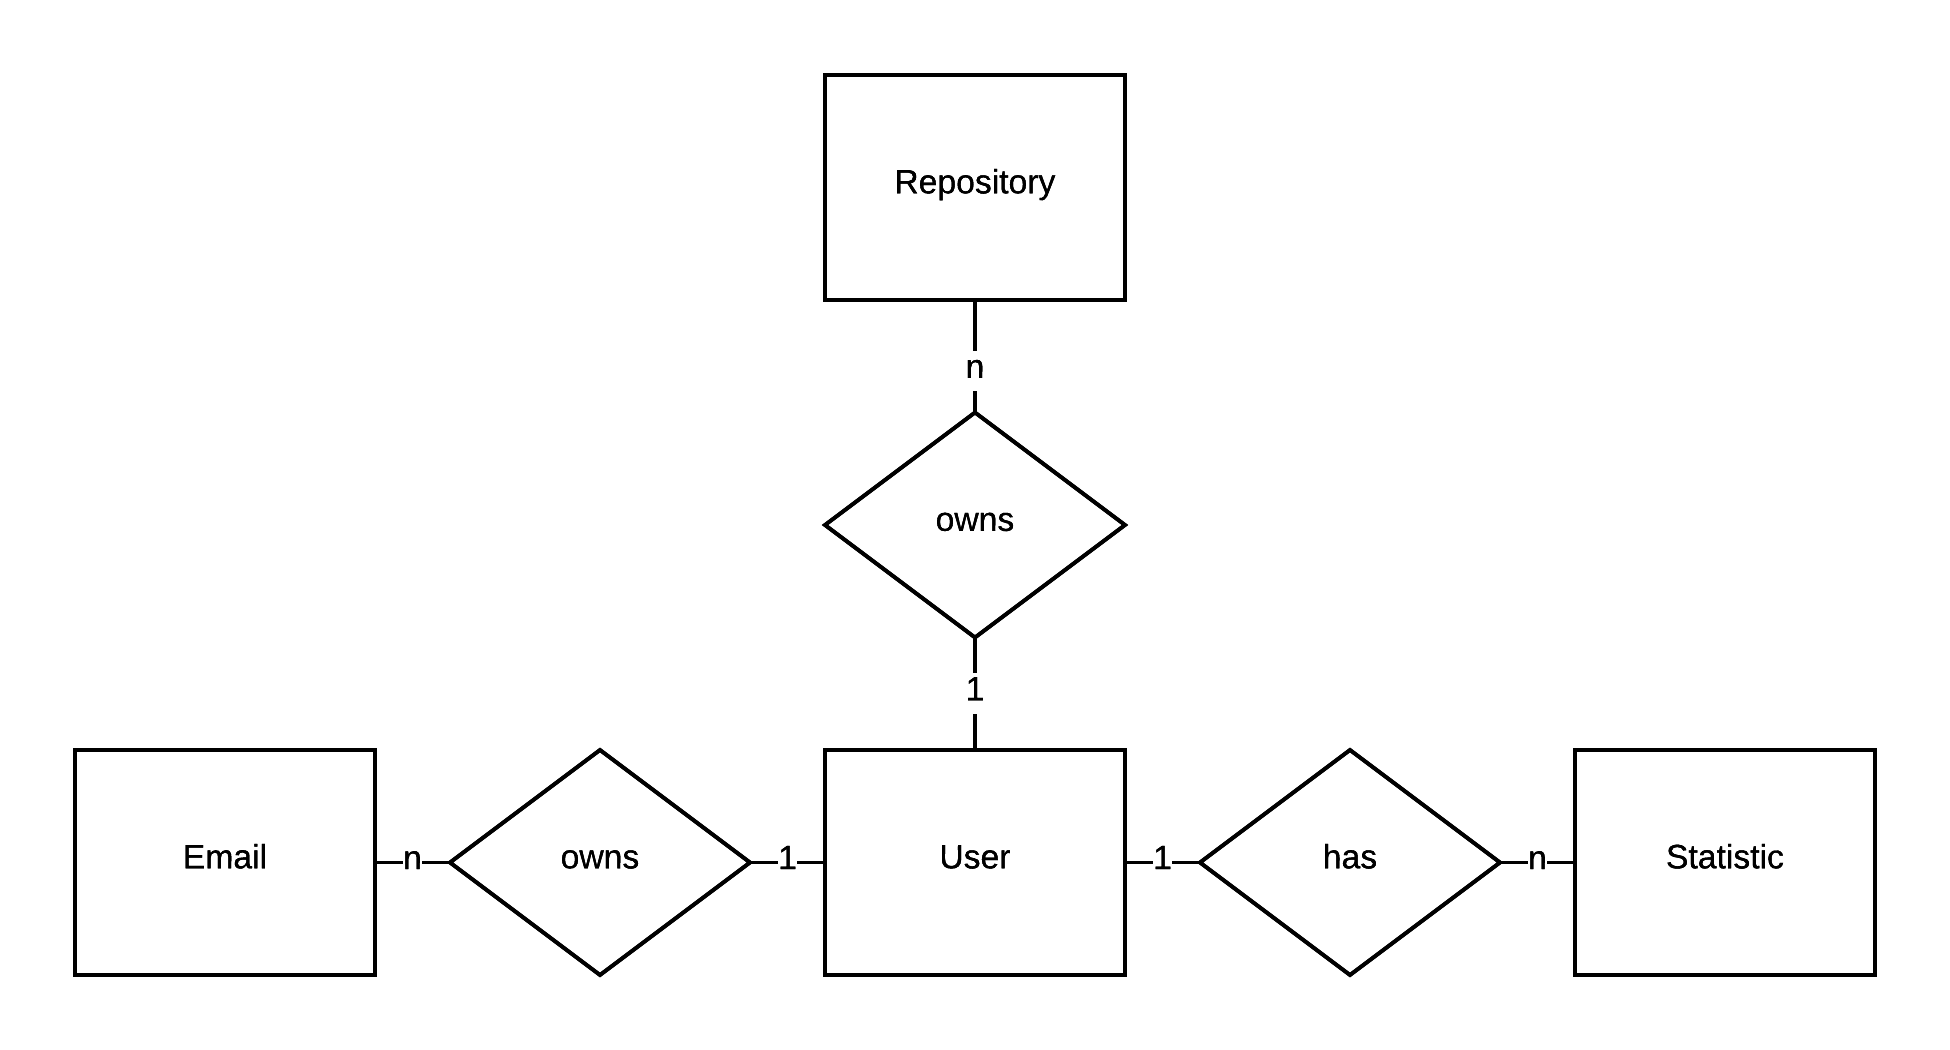
\includegraphics[width=35em]{gfx/schema.png}
  \caption{The hirebot database schema. Only attributes that are mined from the code are listed. To preserve space, attributes are grouped in curly braces if they share prefixes or suffixes}
  \label{fig:schema}
\end{figure}

\subsection{Metric evaluation}
The metric is aggregated from the raw commit analysis data using an SQL view called \verb=calculatedmetric=.

\begin{lstlisting}[language=SQL, frame=false]
CREATE VIEW IF NOT EXISTS calculatedmetric AS
  SELECT userid, language, MIN(date) AS firstcommitdate, MAX(date) AS lastcommitdate, SUM(lines) AS linecount, COUNT(commitid) AS commitcount, julianday(MAX(date)) - julianday(MIN(date)) AS timespan, SUM(lines)/COUNT(commitid) AS averagecommitsize, (julianday(MAX(date)) - julianday(MIN(date)))/COUNT(commitid) AS productivity
  FROM statistics GROUP BY userid, language
  HAVING MIN(date) <> MAX(date)
  ORDER BY userid, timespan DESC, productivity ASC
\end{lstlisting}

Upon querying candidates who suit certain requirement levels, a little logic becomes necessary to build the query. To include candidates in the result set who can provide \textit{some} of the skills, it is necessary to construct combinations of the required programming languages. I.e. if Java, C++ and JavaScript experience levels of at least 3 years were asked for, there would be four combinations, not counting the single options.
Thus, four queries need to be built and executed:

\begin{minipage}{\linewidth}
\begin{lstlisting}[language=SQL, frame=false]
SELECT id,profilename,name,profileurl,avatarurl,location,hireable,followers,following FROM users u
  WHERE 'Java' IN (SELECT language FROM calculatedmetric WHERE userid = u.id AND timespan >= 360*1.5)
    AND 'C++' IN (SELECT language FROM calculatedmetric WHERE userid = u.id AND timespan >= 360*1.5)
    AND 'JavaScript' IN (SELECT language FROM calculatedmetric WHERE userid = u.id AND timespan >= 360*1.5)

SELECT id,profilename,name,profileurl,avatarurl,location,hireable,followers,following FROM users u
  WHERE 'Java' IN (SELECT language FROM calculatedmetric WHERE userid = u.id AND timespan >= 360*1.5)
    AND 'C++' IN (SELECT language FROM calculatedmetric WHERE userid = u.id AND timespan >= 360*1.5)
    AND NOT 'JavaScript' IN (SELECT language FROM calculatedmetric WHERE userid = u.id AND timespan >= 360*1.5)
...
\end{lstlisting}
\end{minipage}

We are aware of the fact that this does not scale well. The queries would perform a lot faster if views were materialized, but SQLITE3 does not offer this commodity. As such response times are a little higher than they should be.

\section{Interface}
\subsection{Candidate view}
A candidate can view his general personal statistics and the JavaScript statistics
mentioned above. This provides him with insight about what job offers he might
receive and what to improve about his coding style (see figure \ref{fig:candidateview})

\begin{figure}
  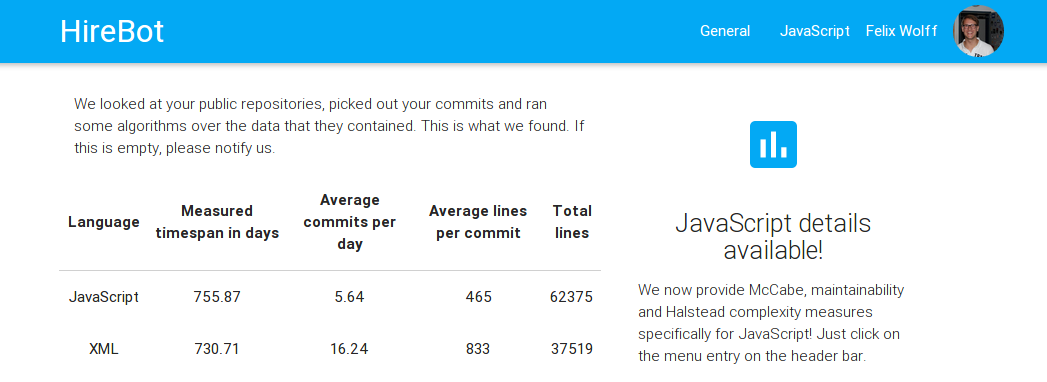
\includegraphics[width=30em]{gfx/candidateview.png}
  \caption{The candidate view of Hirebot}
  \label{fig:candidateview}
\end{figure}

\subsection{Employer view}
In a small small search form, a recruiter can state his requirements concerning
programming language knowledge and for how long this skill should be in training (see figure \ref{fig:employerview}).

\begin{figure}
  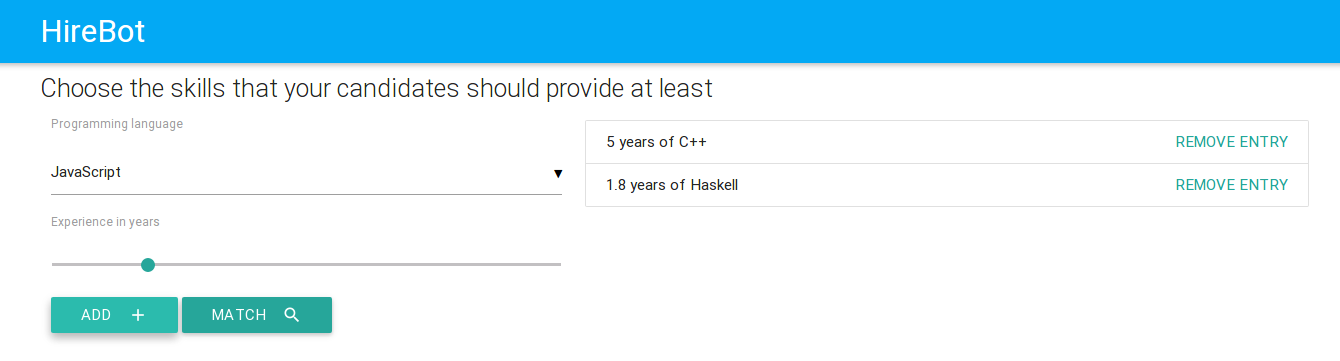
\includegraphics[width=30em]{gfx/employerview.png}
  \caption{The employer search form of Hirebot}
  \label{fig:employerview}
\end{figure}
